\chapter{Entwicklung eines technischen Objekts}
%TODO Einleitung: Idee
% explizite Bezug auf Ultimaker 2, andere Drucker liefern andere Ergebnisse

Dieses Kapitel handelt vom Entwerfen und Drucken eines technischen Objekts. Als Objekt wird hier exemplarisch ein Aufbewahrungssystem f�r einen Raspberry Pi gekoppelt mit einem \ac{USB}- Hub und einer  externen Festplatte entworfen. Dieses System soll m�glichst kompakt sein und als ein Block transportierbar sein.

Diese Arbeit bezieht sich h�ufig auf den ultimaker 2, der im vorhergehenden Kapitel \ref{chapter:techGr:ultimaker2} vorgestellt wird. In der Arbeit mit einem anderen Drucker k�nnen sich Vorgehensweise und Ergebnis deutlich unterscheiden.

Zuerst wird die Analyse der bestehenden Verwahrung beschrieben. Anschlie�end folgt eine Beschreibung des umzusetzenden Konzepts. Folgend wird ein Entwurf des Systems mit einem \ac{CAD}-Programm  und der Druck des Objekts beschrieben. Der darauffolgende Abschnitt besch�ftigt sich mit w�hrend dem Druck aufgetretenen Fehlern. Zuletzt folgt ein Fazit �ber die Eignung des ultimaker 2 zum Drucken von technischen Objekten.


%TODO Ist-Analyse
\newpage
\section{Ist-Analyse}
	\piccaption{Urspr�ngliches Stapelsystem}
	\parpic{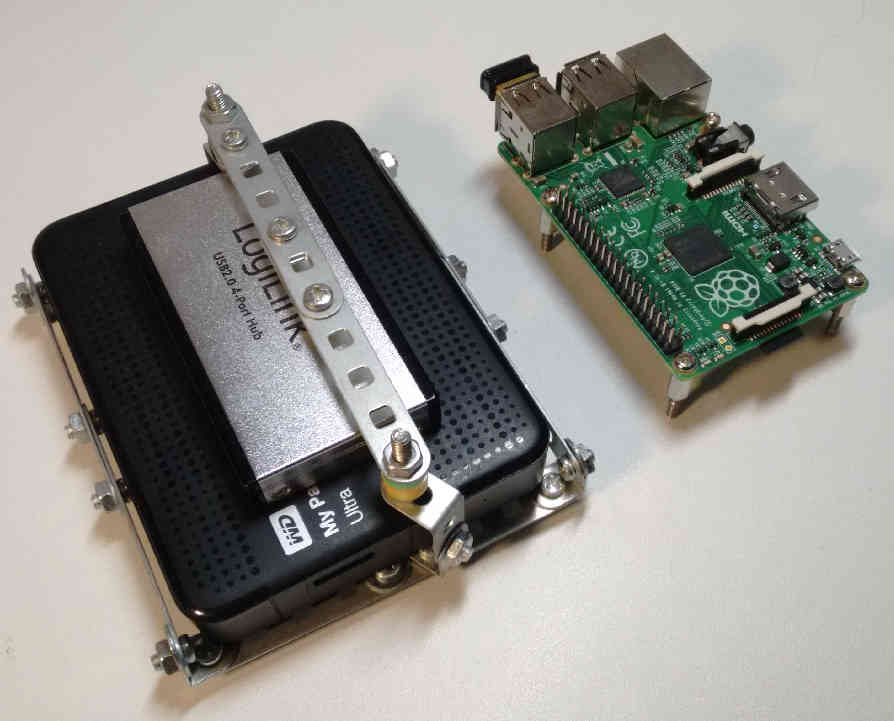
\includegraphics[width=.5\textwidth]{images/techObj/urspruenglicheHalterung02.jpg}}
	
	\picskip{0}
	
%TODO 
\section{Konzept: Modulare Boxen}

\section{Entwurf}
%Erw�hnen, dass Solid Edge verwendet

\section{Druck des Objekts}
% Wie w�re es ideal gewesen?, fertiges Objekt 
% Welche Parameter? --> spezifisch beim technischen Objekt
% Verlinkung zu Fehlern

\section{Aufgetretene Fehler}
% Bilder
% Fehleranalyse, [Ma�nahmen --> technische Grundlagen]

\section{Fazit: Eignung f�r technische Objekte}
% bezogen auf Ultimaker